% Chapter 1

\chapter{Introducción general} % Main chapter title

\label{Chapter1} % For referencing the chapter elsewhere, use \ref{Chapter1} 
\label{IntroGeneral}

%----------------------------------------------------------------------------------------

% Define some commands to keep the formatting separated from the content 
\newcommand{\keyword}[1]{\textbf{#1}}
\newcommand{\tabhead}[1]{\textbf{#1}}
\newcommand{\code}[1]{\texttt{#1}}
\newcommand{\file}[1]{\texttt{\bfseries#1}}
\newcommand{\option}[1]{\texttt{\itshape#1}}
\newcommand{\grados}{$^{\circ}$}

En este capítulo se presenta el marco de referencia y la justificación del proyecto titulado Modernización de contadores de tránsito con comunicación bidireccional. Se expone el contexto que motivó la intervención, se describen los problemas detectados en la infraestructura vigente, se revisa el estado del arte y la propuesta de valor del trabajo, y se delimita el alcance del prototipo propuesto. El objetivo es proporcionar al lector una visión global que permita comprender las decisiones de diseño y los criterios de priorización adoptados en las etapas siguientes del trabajo.
%----------------------------------------------------------------------------------------

%\section{Introducción}

%----------------------------------------------------------------------------------------
\newpage

\section{Introducción y motivación}

Este trabajo propone la modernización de los contadores de tránsito instalados en rutas nacionales mediante la renovación de su arquitectura de comunicaciones. Actualmente los equipos registran el paso de vehículos y transmiten eventos al servidor central a través de enlaces GPRS tercerizados. Sin embargo, no admiten la recepción de comandos ni la obtención de diagnósticos remotos. Dicha limitación reduce la capacidad operativa, incrementa los costos de mantenimiento y demora la resolución de fallas, pues cualquier ajuste o reparación exige intervención presencial.

El objetivo general del proyecto es diseñar y construir un prototipo, Producto Mínimo Viable (MVP), que garantice la transmisión segura y confiable de los datos de tránsito y que habilite la gestión remota de los equipos en campo. Para ese propósito se plantean metas concretas. 
En primer lugar se busca asegurar la entrega de eventos aun cuando la conectividad sea intermitente. En segundo lugar se propone implementar mecanismos de encolamiento y reintento en el dispositivo que eviten duplicados y pérdidas de información y en tercer lugar se pretende habilitar la ejecución remota de comandos y la actualización de parámetros desde un servidor central con confirmación explícita del estado del equipo.

Los objetivos específicos apuntan a incrementar la autonomía operativa de la institución y a reducir costos recurrentes asociados a la dependencia de proveedores externos de conectividad. En particular, el proyecto aspira a: 
\begin{itemize}
\item Disminuir la dependencia de enlaces tercerizados mediante una arquitectura configurable

\item Permitir la modificación remota de parámetros operativos y la carga de ajustes sin requerir desplazamientos 

\item Incorporar telemetría de estado (nivel de batería, temperatura y códigos de error) para facilitar el mantenimiento preventivo

\item Validar mediante el MVP la viabilidad técnica, la robustez operativa y los beneficios económicos de la propuesta.
\end{itemize}

El alcance técnico del MVP incluye la adaptación de un contador existente para comunicarse bidireccionalmente por GPRS, que emplee MQTT como protocolo de mensajería ligera y confiable. Asimismo, comprende el desarrollo de un backend que reciba, procese y persista los eventos en una base de datos relacional. Además una interfaz web básica que permita la visualización en tiempo real y el envío de comandos hacia los dispositivos. Se priorizarán las funciones que validen la cadena completa: adquisición de eventos desde el sistema de detección, encolamiento local con política FIFO, reenvío seguro cuando haya conectividad, recepción y ejecución de comandos y verificación del estado del dispositivo tras cada acción.

Desde la perspectiva de operación y mantenimiento, la modernización busca reducir los desplazamientos de personal técnico y acortar los tiempos de resolución de incidentes, con la consiguiente disminución de costos logísticos. La incorporación de telemetría permitirá planificar intervenciones preventivas en lugar de responder exclusivamente a fallas, lo que mejorará la disponibilidad del servicio y la calidad de los datos recolectados. Además, la adopción de protocolos estandarizados y componentes de código abierto promoverá la escalabilidad y la replicabilidad de la solución en distintos tramos de la red vial.

Por último, la propuesta separa de forma explícita el transporte de mensajes (broker MQTT) de los servicios de aplicación (API REST, almacenamiento y frontend). Esta separación facilita la interoperabilidad con plataformas institucionales existentes y habilita opciones de despliegue flexibles: uso de brokers externos, instalación de brokers locales o modelos híbridos según políticas institucionales y condiciones de conectividad. En síntesis, el proyecto busca ofrecer una solución técnica y económica que permita gestionar de manera proactiva y eficiente la infraestructura de conteo de tránsito proporcionando una base verificable para su posterior escalado e integración institucional.


%----------------------------------------------------------------------------------------
\newpage

\section{Problemas identificados}

El análisis del sistema vigente permitió identificar las siguientes limitaciones que motivan el rediseño:

\begin{itemize}
\item  Comunicación unidireccional. Los contadores envían datos al servidor pero no existe un canal para enviar configuraciones, consultas y comandos desde el servidor hacia los equipos. Esta limitación impide realizar diagnósticos remotos y ejecutar acciones correctivas sin presencia física.

\item  Dependencia de proveedores GPRS tercerizados. La dependencia de servicios contratados genera costos recurrentes y limita el control sobre la calidad y disponibilidad de la conectividad.

\item  Imposibilidad de actualización remota. Cualquier modificación de parámetros o ajustes de operación requiere intervención en el sitio. Esto incrementa tiempos de mantenimiento y costos logísticos y complica la aplicación rápida de mejoras.

\item  Falta de telemetría y diagnóstico preventivo. No se dispone de métricas sistemáticas sobre la salud de los equipos (batería, temperatura, errores de hardware o comunicación).

\item Riesgo de pérdida de datos ante conectividad intermitente. La ausencia de mecanismos de encolamiento persistente y de políticas claras de reenvío eleva la probabilidad de pérdida o duplicación de eventos cuando la red es inestable.

\end{itemize}

Estas deficiencias afectan la calidad del servicio de monitoreo, reducen la eficiencia operativa y constituyen los requisitos funcionales que orientan el diseño del prototipo: comunicación bidireccional segura, encolamiento local con política FIFO, reintentos controlados, autenticación en el broker MQTT y telemetría de estado.


--------------------------------------------------------------------------------------
\newpage

\section{Estado del arte y propuesta de valor}

En el mercado existen soluciones comerciales que ofrecen gestión remota y comunicación bidireccional para dispositivos de campo. Dichas soluciones suelen incluir plataformas propietarias con soporte, servicio administrado y herramientas de análisis. No obstante, su adopción conlleva costos elevados y, en muchos casos, dependencias tecnológicas que dificultan la adaptación a especificidades locales.

La propuesta de este trabajo adopta un enfoque alternativo: emplear tecnologías de código abierto y protocolos estandarizados, especialmente MQTT, para construir una arquitectura flexible, escalable y de bajo costo. La separación entre el transporte de mensajes (broker MQTT) y los servicios de aplicación (API REST, base de datos y frontend) facilita la interoperabilidad y permite operar con brokers locales o externos según requieran las políticas institucionales.

Adicionalmente, la solución incorpora mecanismos diseñados para condiciones operativas típicas de rutas nacionales: operación con conectividad intermitente, envío diferido con políticas FIFO, control de reintentos para evitar duplicados y autenticación de credenciales en el broker MQTT. Este conjunto de medidas asegura integridad y trazabilidad de los eventos sin depender exclusivamente de servicios propietarios.

El valor diferencial reside en ofrecer una alternativa económicamente viable que preserve funcionalidad y escalabilidad, y que a su vez permita a la institución mantener control operativo sobre la infraestructura. La propuesta facilita la migración progresiva desde soluciones tercerizadas hacia una plataforma propia o semi-autónoma, reduciendo costos recurrentes y mejorando la capacidad de respuesta ante incidentes.

\newpage

\section{Alcance}
El proyecto desarrollará un prototipo funcional destinado a validar las hipótesis técnicas y operativas. El alcance comprende los siguientes entregables y límites:

\begin{itemize}

\item Rediseño de comunicaciones: implementación de un modelo bidireccional y seguro entre los dispositivos de conteo y el servidor central, basado en MQTT sobre GPRS y con autenticación por credenciales.

\item Gestión de mensajes en el dispositivo: encolamiento en memoria RAM con política FIFO, control de reintentos ante fallos de conexión y lógica de descarte cuando la cola alcance su límite definido.

\item Backend y persistencia: desarrollo de una API REST que se suscriba al broker MQTT, procese los eventos y almacene los registros en una base de datos relacional para consulta histórica.

\item Interfaz web básica: panel de visualización en tiempo real de eventos de tránsito y módulo para envío de comandos y verificación de estado de los dispositivos.

\item Funciones de telemetría: reporte de nivel de batería, temperatura y códigos de error para facilitar el diagnóstico remoto.

\item  Fuera del alcance del MVP: implementación de algoritmos avanzados de inteligencia artificial para estimación o reconstrucción de tránsitos no detectados, el despliegue masivo en toda la red de rutas ni la creación de una plataforma comercial completa con soporte SLAs. El propósito es validar los componentes esenciales que permitan, en etapas posteriores, escalar la solución e incorporar servicios adicionales.
\end{itemize}

La figura 1 muestra el diagrama en bloques del sistema. El dispositivo de conteo envía datos por GPRS a un broker MQTT; el servidor central los procesa y almacena en una base de datos, mientras que una API REST permite su consulta y la ejecución de comandos desde una interfaz web.

\vspace{1cm}

\begin{figure}[htbp]
	\centering
	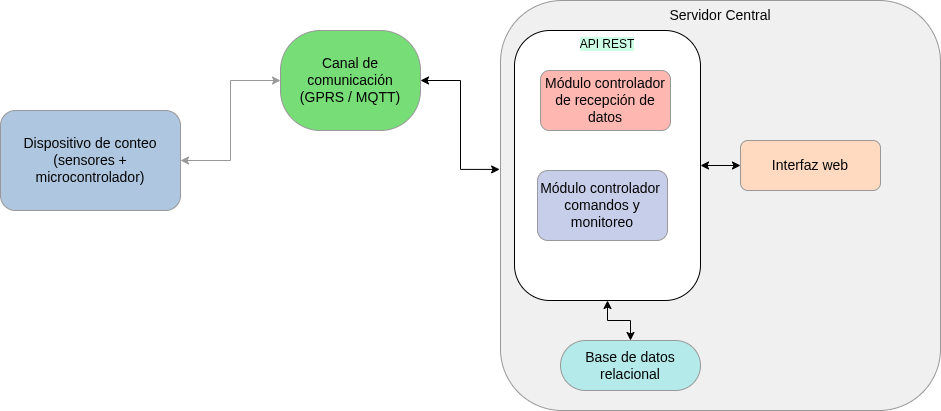
\includegraphics[width=.98\textwidth]{./Figures/diagBloques.png}
	\caption{Diagrama de bloques.}
	\label{fig:texmaker}
\end{figure}

\vspace{1cm}











